\documentclass[journal,12pt,twocolumn]{IEEEtran}

\usepackage{setspace}
\usepackage{gensymb}
\singlespacing
\usepackage[cmex10]{amsmath}

\usepackage{amsthm}

\usepackage{mathrsfs}
\usepackage{txfonts}
\usepackage{stfloats}
\usepackage{bm}
\usepackage{cite}
\usepackage{cases}
\usepackage{subfig}

\usepackage{longtable}
\usepackage{multirow}
\usepackage{graphicx}
\usepackage{enumitem}
\usepackage{mathtools}
\usepackage{steinmetz}
\usepackage{tikz}
\usepackage{circuitikz}
\usepackage{verbatim}
\usepackage{tfrupee}
\usepackage[breaklinks=true]{hyperref}
\usepackage{graphicx}
\usepackage{tkz-euclide}
\usepackage{amsmath}
\usetikzlibrary{calc,math}
\usepackage{listings}
    \usepackage{color}                                            %%
    \usepackage{array}                                            %%
    \usepackage{longtable}                                        %%
    \usepackage{calc}                                             %%
    \usepackage{multirow}                                         %%
    \usepackage{hhline}                                           %%
    \usepackage{ifthen}                                           %%
    \usepackage{lscape}     
\usepackage{multicol}
\usepackage{chngcntr}

\DeclareMathOperator*{\Res}{Res}

\renewcommand\thesection{\arabic{section}}
\renewcommand\thesubsection{\thesection.\arabic{subsection}}
\renewcommand\thesubsubsection{\thesubsection.\arabic{subsubsection}}

\renewcommand\thesectiondis{\arabic{section}}
\renewcommand\thesubsectiondis{\thesectiondis.\arabic{subsection}}
\renewcommand\thesubsubsectiondis{\thesubsectiondis.\arabic{subsubsection}}

\graphicspath{{figures/}}

\hyphenation{op-tical net-works semi-conduc-tor}
\def\inputGnumericTable{}                                 %%

\lstset{
%language=C,
frame=single, 
breaklines=true,
columns=fullflexible
}
\begin{document}


\newtheorem{theorem}{Theorem}[section]
\newtheorem{problem}{Problem}
\newtheorem{proposition}{Proposition}[section]
\newtheorem{lemma}{Lemma}[section]
\newtheorem{corollary}[theorem]{Corollary}
\newtheorem{example}{Example}[section]
\newtheorem{definition}[problem]{Definition}

\newcommand{\BEQA}{\begin{eqnarray}}
\newcommand{\EEQA}{\end{eqnarray}}
\newcommand{\define}{\stackrel{\triangle}{=}}
\bibliographystyle{IEEEtran}
\raggedbottom
\setlength{\parindent}{0pt}
\providecommand{\mbf}{\mathbf}
\providecommand{\pr}[1]{\ensuremath{\Pr\left(#1\right)}}
\providecommand{\qfunc}[1]{\ensuremath{Q\left(#1\right)}}
\providecommand{\sbrak}[1]{\ensuremath{{}\left[#1\right]}}
\providecommand{\lsbrak}[1]{\ensuremath{{}\left[#1\right.}}
\providecommand{\rsbrak}[1]{\ensuremath{{}\left.#1\right]}}
\providecommand{\brak}[1]{\ensuremath{\left(#1\right)}}
\providecommand{\lbrak}[1]{\ensuremath{\left(#1\right.}}
\providecommand{\rbrak}[1]{\ensuremath{\left.#1\right)}}
\providecommand{\cbrak}[1]{\ensuremath{\left\{#1\right\}}}
\providecommand{\lcbrak}[1]{\ensuremath{\left\{#1\right.}}
\providecommand{\rcbrak}[1]{\ensuremath{\left.#1\right\}}}
\theoremstyle{remark}
\newtheorem{rem}{Remark}
\newcommand{\sgn}{\mathop{\mathrm{sgn}}}
\providecommand{\abs}[1]{\left\vert#1\right\vert}
\providecommand{\res}[1]{\Res\displaylimits_{#1}} 
\providecommand{\norm}[1]{\left\lVert#1\right\rVert}
%\providecommand{\norm}[1]{\lVert#1\rVert}
\providecommand{\mtx}[1]{\mathbf{#1}}
\providecommand{\mean}[1]{E\left[ #1 \right]}
\providecommand{\fourier}{\overset{\mathcal{F}}{ \rightleftharpoons}}
%\providecommand{\hilbert}{\overset{\mathcal{H}}{ \rightleftharpoons}}
\providecommand{\system}{\overset{\mathcal{H}}{ \longleftrightarrow}}
	%\newcommand{\solution}[2]{\textbf{Solution:}{#1}}
\newcommand{\solution}{\noindent \textbf{Solution: }}
\newcommand{\cosec}{\,\text{cosec}\,}
\providecommand{\dec}[2]{\ensuremath{\overset{#1}{\underset{#2}{\gtrless}}}}
\newcommand{\myvec}[1]{\ensuremath{\begin{pmatrix}#1\end{pmatrix}}}
\newcommand{\mydet}[1]{\ensuremath{\begin{vmatrix}#1\end{vmatrix}}}
\numberwithin{equation}{subsection}
\makeatletter
\@addtoreset{figure}{problem}
\makeatother
\let\StandardTheFigure\thefigure
\let\vec\mathbf
\renewcommand{\thefigure}{\theproblem}
\def\putbox#1#2#3{\makebox[0in][l]{\makebox[#1][l]{}\raisebox{\baselineskip}[0in][0in]{\raisebox{#2}[0in][0in]{#3}}}}
     \def\rightbox#1{\makebox[0in][r]{#1}}
     \def\centbox#1{\makebox[0in]{#1}}
     \def\topbox#1{\raisebox{-\baselineskip}[0in][0in]{#1}}
     \def\midbox#1{\raisebox{-0.5\baselineskip}[0in][0in]{#1}}
\vspace{3cm}
\title{Assignment 2}
\author{Vaddamani Saketh - CS20BTECH11054}
\maketitle
\newpage
\bigskip
\renewcommand{\thefigure}{\theenumi}
\renewcommand{\thetable}{\theenumi}
Download all python codes from 
\begin{lstlisting}
https://github.com/CS20BTECH11054/AI1103/blob/main/Assignment_2/codes/Assignment_2.py
\end{lstlisting}
%
and latex-tikz codes from 
%
\begin{lstlisting}
https://github.com/CS20BTECH11054/AI1103/blob/main/Assignment_2/Assignment_2.tex
\end{lstlisting}
\section{Problem}
(Prob, 5.30) Find the variance of the number obtained on a throw of an unbiased die
\section{Solution}
Let $X \in \{1,2,3,4,5,6\}$, be the random variable representing outcome of the die.The probability mass function(pmf) can be expressed as
\begin{align}
p_X(n) = P(X=n) =    \left\{
                  \begin{array}{ll}
                      \frac{1}{6} & 1 \leq n \leq 6 \\
                      0 & otherwise \\
                  \end{array} 
                  \right.    
\end{align}
The variance (Var(X)) of this distribution can be found by definition,\\
\begin{align}
Var(X) = E(X^{2})-(E(X))^{2}
\end{align}
where,
\begin{align}
E(X)=\sum_{k=1}^{k=6} kp_X(k)\\
E(X)=\frac{1}{6}\sum_{k=1}^{k=6} k\\
E(X)=\frac{1}{6} \times \frac{6\times7}{2}\\
E(X)=\frac{7}{2}
\end{align}
\\
\begin{align}
E(X^{2})=\sum_{k=1}^{k=6} k^{2}p_X(k)\\
E(X^{2})=\frac{1}{6}\sum_{k=1}^{k=6} k^{2}\\
E(X^{2})=\frac{1}{6} \times \frac{6\times7\times13}{6}\\
E(x^{2})=\frac{91}{6}
\end{align}
Therefore, substituting values from Eq.(2.0.6) and Eq.(2.0.10), we get
\begin{align}
Var(X) = E(X^{2})-(E(X))^{2}\\
Var(X) = \frac{91}{6} - \frac{49}{4}\\
Var(X) = \frac{70}{12}\\
Var(X) = 2.9167
\end{align}
Therefore, the variance of the number obtained on a throw of an unbiased die is \textbf{2.9167}.
\newpage
\begin{figure}
    \centering
    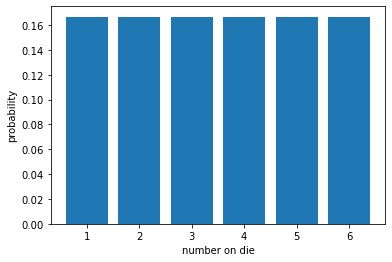
\includegraphics[width=18cm]{Assignment_2.png}
\end{figure}
\end{document}
